\documentclass{ieeetj}
\usepackage{cite}
\usepackage{amsmath,amssymb,amsfonts}
\usepackage{algorithmic}
\usepackage{graphicx,color}
\usepackage{textcomp}
\usepackage{xcolor}
\usepackage{hyperref}
\hypersetup{hidelinks=true}
\usepackage{algorithm,algorithmic}
\usepackage{tikz}
\usetikzlibrary{shapes,arrows,positioning,calc,shadows,decorations.pathmorphing}
\def\BibTeX{{\rm B\kern-.05em{\sc i\kern-.025em b}\kern-.08em
    T\kern-.1667em\lower.7ex\hbox{E}\kern-.125emX}}
\AtBeginDocument{\definecolor{tmlcncolor}{cmyk}{0.93,0.59,0.15,0.02}\definecolor{NavyBlue}{RGB}{0,86,125}}




\def\OJlogo{\vspace{-17pt}
\includegraphics[width=3.5cm]{img/banner.png}}
\def\seclogo{\vspace{-4pt}
\includegraphics[width=3.5cm]{img/banner.png}}
\jvol{1}

\def\authorrefmark#1{\ensuremath{^{\textbf{#1}}}}

% Redefinici\'on del entorno abstract para soporte biling\"ue (Resumen + Abstract)
% Se elimina el encabezado ABSTRACT autom\'atico de la clase para insertar
% los encabezados manualmente en el orden deseado.
\def\abstract{%
  \global\setbox\abstractbox\vbox\bgroup
  \parindent0pt\hsize\textwidth\abstractfont\ignorespaces}
\def\endabstract{\egroup}

\begin{document}
\receiveddate{22 March, 2026}
\reviseddate{22 March, 2026}
\accepteddate{22 March, 2026}
\publisheddate{22 March, 2026}
\currentdate{22 March, 2026}
\doiinfo{}

\markboth{}{Quintero Rubiano}

\title{LUCID: Un Framework de IA Generativa para la Gamificación Matemática Adaptativa}

\author{Juan Carlos Quintero Rubiano}
\affil{Estudiante de Ingenier\'ia de Sistemas, Universidad Distrital -- C\'odigo de estudiante 20232020172}
\corresp{Corresponding author: Juan Carlos Quintero Rubiano (email: jcquinteror@udistrital.edu.co).}


\begin{abstract}
{\abstractheadfont\bfseries\textcolor{tmlcncolor}{RESUMEN}}\hspace*{3pt}%
LUCID es un framework de software basado en Inteligencia Artificial Generativa dise\~nado para
abordar una problem\'atica profunda en la educaci\'on de j\'ovenes: la tendencia de los
adolescentes a memorizar f\'ormulas y procedimientos matem\'aticos sin comprender los conceptos
que los sustentan, lo que genera un aprendizaje fr\'agil, ansiedad ante la evaluaci\'on y una
relaci\'on negativa con la matem\'atica desde etapas tempranas de su formaci\'on.
En lugar de presentar la aritm\'etica y la l\'ogica como reglas abstractas a reproducir
mec\'anicamente, LUCID transforma cada concepto en un desaf\'io narrativo dentro de un mundo
de rol generado proceduralmente, donde el estudiante debe razonar y construir la soluci\'on
para hacer avanzar la historia, no simplemente aplicar una f\'ormula memorizada.
El sistema emplea Modelos de Lenguaje de Gran Escala~(LLMs) como motor narrativo que act\'ua
como un ``Dungeon Master'' digital, adaptando los retos al nivel conceptual real de cada
usuario con base en su historial de aciertos y errores, con el objetivo de cerrar la brecha
entre el procedimiento mec\'anico y la comprensi\'on genuina.
Un microservicio de validaci\'on simb\'olica implementado con Python/SymPy verifica la
correcci\'on matem\'atica de las respuestas y previene alucinaciones de la IA, garantizando
que el contenido generado sea pedag\'ogicamente \'integro.
De esta forma, LUCID propone la Generaci\'on Procedural de Contenido~(PCG) como una herramienta
escalable para reemplazar la memorizaci\'on pasiva por una comprensi\'on activa y significativa
de la matem\'atica en j\'ovenes estudiantes.

\smallskip\noindent
{\abstractheadfont\bfseries\textcolor{tmlcncolor}{T\'ERMINOS DE INDEXADO}}\hspace*{3pt}%
\textit{adolescentes, aprendizaje adaptativo, aprendizaje basado en juegos, comprensi\'on conceptual,
educaci\'on matem\'atica, gamificaci\'on, generaci\'on procedural de contenido,
inteligencia artificial generativa, juegos serios, modelos de lenguaje de gran escala.}

\bigskip\noindent
{\abstractheadfont\bfseries\textcolor{tmlcncolor}{ABSTRACT}}\hspace*{3pt}%
LUCID is a generative artificial intelligence framework designed to address a pervasive problem
in secondary education: the tendency of adolescent students to memorize mathematical formulas
and procedures without understanding the underlying concepts, resulting in fragile knowledge,
evaluation anxiety, and a lasting negative relationship with mathematics.
Rather than presenting arithmetic and logical reasoning as abstract rules to be mechanically
reproduced, LUCID embeds each concept within a procedurally generated role-playing narrative
where students must reason through problems to advance the story---replacing passive recall
with active conceptual construction.
The system deploys large language models~(LLMs) as a digital Dungeon Master that generates
contextually coherent mathematical challenges adapted in real time to each learner's conceptual
profile, inferred from their history of correct and incorrect responses, targeting the gap
between procedural execution and genuine understanding.
A symbolic validation microservice built with Python/SymPy acts as a mathematical truth oracle,
verifying the correctness of user answers and preventing AI hallucinations, thereby ensuring
the pedagogical integrity of all generated content.
A procedural adaptability algorithm adjusts both narrative tone and challenge difficulty to
maintain each student in a state of cognitive flow, progressively replacing formula-dependent
thinking with deep conceptual reasoning.
Evaluation objectives include AI response latency benchmarking and student-perception surveys
measuring the reduction of rote memorization dependency and mathematical anxiety compared to
traditional instructional methods.
LUCID represents a convergence of serious game design, generative AI, and constructivist
pedagogy aimed at transforming how young learners build mathematical understanding from the
ground up.
\end{abstract}

\begin{IEEEkeywords}
adolescents, adaptive learning, conceptual understanding, game-based learning,
gamification, generative artificial intelligence, large language models,
mathematical education, procedural content generation, serious games.
\end{IEEEkeywords}

%\IEEEspecialpapernotice{(Invited Paper)}

\maketitle

\section{INTRODUCCIÓN}
\IEEEPARstart{L}a ense\~nanza de las matem\'aticas en la educaci\'on secundaria enfrenta desaf\'ios
sist\'emicos relacionados con la desvinculaci\'on cognitiva de los estudiantes. La tendencia a
priorizar la memorizaci\'on de procedimientos algor\'itmicos sobre la comprensi\'on conceptual
profunda ha generado un fen\'omeno de aprendizaje superficial, caracterizado por altos \'indices
de ansiedad acad\'emica y una transferencia deficiente del conocimiento~\cite{estrada2024impacto}.
Para mitigar esta problem\'atica, la investigaci\'on educativa reciente ha convergido en dos
paradigmas tecnol\'ogicos: la gamificaci\'on de los entornos de aprendizaje y la integraci\'on
de sistemas de Inteligencia Artificial~(IA) adaptativa.

La gamificaci\'on, definida como la aplicaci\'on de elementos de dise\~no de juegos en contextos
no l\'udicos, ha demostrado ser un catalizador eficaz para la motivaci\'on intr\'inseca.
Ahma y Kadriu~\cite{ahma2025exploring} evaluaron el impacto de diversas estrategias gamificadas,
concluyendo que estas proporcionan ``informaci\'on valiosa para educadores y responsables
pol\'iticos que buscan incorporar la gamificaci\'on en sus estrategias de ense\~nanza, con el
objetivo final de crear entornos m\'as atractivos''. No obstante, su aplicaci\'on en dominios
altamente estructurados como las matem\'aticas presenta limitaciones. En su revisi\'on
sistem\'atica orientada a ``reportar las tendencias actuales de implementaci\'on de la
gamificaci\'on en la educaci\'on matem\'atica secundaria'', Mayrhofer et al.~\cite{mayrhofer2025current}
identificaron que la mayor\'ia de las arquitecturas actuales se basan en sistemas de
recompensas extr\'insecas (puntos e insignias) superpuestos a curr\'iculos est\'aticos.
Esta falta de integraci\'on estructural es corroborada por Mar\'in y Cantillo~\cite{marin2025gamificacion},
quienes se\~nalan que la ausencia de retroalimentaci\'on din\'amica provoca una r\'apida
obsolescencia del est\'imulo l\'udico.

La incorporaci\'on de IA ofrece un mecanismo para superar la rigidez de la gamificaci\'on
tradicional. Suresh Babu y Dhakshina Moorthy~\cite{suresh2024application} establecen que la
ventaja competitiva de la IA radica en su capacidad para la personalizaci\'on algor\'itmica
del contenido. Gunawan et al.~\cite{gunawan2025future} expanden esta premisa, argumentando
que los modelos generativos posibilitan la s\'intesis de experiencias educativas en tiempo real.
En este contexto, los Modelos de Lenguaje de Gran Escala~(LLMs) han emergido como tutores
cognitivos viables. Adewumi et al.~\cite{adewumi2025findings} validaron emp\'iricamente la
``explicaci\'on matem\'atica con LLMs utilizando el m\'etodo socr\'atico para el aprendizaje
activo'', demostrando que la IA puede andamiar el proceso de resoluci\'on de problemas
mediante interrogaci\'on guiada, en lugar de la provisi\'on directa de respuestas.

A pesar de estos avances, persiste una brecha arquitect\'onica en la literatura: la ausencia
de frameworks que integren org\'anicamente la generaci\'on procedural de narrativas, la
tutor\'ia socr\'atica basada en LLMs y mecanismos deterministas de validaci\'on matem\'atica.
Los sistemas actuales carecen del anclaje narrativo necesario para contextualizar la
abstracci\'on matem\'atica o, por el contrario, adolecen de m\'etodos de verificaci\'on
simb\'olica que mitiguen las alucinaciones inherentes a los modelos generativos.

Para abordar esta limitaci\'on, este art\'iculo presenta LUCID~(\textit{Large-language-model
Unified Curriculum Intelligent Designer}), una arquitectura de software que transforma la
resoluci\'on de problemas matem\'aticos en desaf\'ios narrativos dentro de un entorno de rol
generado proceduralmente. El sistema emplea un LLM como motor de adaptabilidad pedag\'ogica
y un microservicio de validaci\'on simb\'olica (Python/SymPy) para garantizar la precisi\'on
matem\'atica. El resto del documento se estructura de la siguiente manera: la Secci\'on~II
presenta los trabajos relacionados y su contraste con este proyecto; la Secci\'on~III detalla
la arquitectura del sistema; la Secci\'on~IV describe el algoritmo de adaptabilidad;
la Secci\'on~V expone la metodolog\'ia de evaluaci\'on; y la Secci\'on~VI agrupa las
conclusiones.

\section{TRABAJOS RELACIONADOS}
La propuesta de LUCID se fundamenta en recientes avances interdisciplinarios que intersectan
la gamificaci\'on educativa, los sistemas adaptativos y la Inteligencia Artificial Generativa.
A continuaci\'on, se analiza la literatura pertinente, destacando los aportes integrables a
nuestro modelo y las limitaciones que esta arquitectura aspira a superar.

\subsection{De la Gamificaci\'on Est\'atica al Dise\~no Narrativo}
La eficacia base de la gamificaci\'on para mitigar la ansiedad acad\'emica~\cite{estrada2024impacto}
y fomentar la motivaci\'on intr\'inseca est\'a extensamente documentada. Estudios como el de
Ahma y Kadriu~\cite{ahma2025exploring} demuestran c\'omo los entornos inmersivos retienen la atenci\'on del
estudiante a corto plazo. Sin embargo, revisiones sistem\'aticas recientes exponen su estancamiento:
Mayrhofer et al.~\cite{mayrhofer2025current} evidenciaron que prevalecen los sistemas extr\'insecos
basados en tablas de clasificaci\'on e insignias (PBL - \textit{Points, Badges, Leaderboards}),
aplicados sobre m\'odulos curriculares est\'aticos. En esta misma l\'inea, Mar\'in y Cantillo~\cite{marin2025gamificacion}
advierten que estos est\'imulos r\'apidamente generan tolerancia y desvinculaci\'on en adolescentes
si carecen de dinamismo. Este comportamiento tambi\'en es consistente con la revisi\'on emp\'irica
de Hamari et al.~\cite{hamari2014does}, donde se reporta que los efectos de la gamificaci\'on
dependen de forma cr\'itica del contexto pedag\'ogico y del dise\~no de interacci\'on.
\textit{Aporte y Contraste:} Estos hallazgos validan la necesidad de abandonar los sistemas de 
recompensas superficiales. En claro contraste con las plataformas evaluadas en~\cite{mayrhofer2025current,marin2025gamificacion},
LUCID prescinde de medallas o r\'ankings extr\'insecos y emplea en su lugar Generaci\'on Procedural 
de Contenido~(PCG) para embeber la operaci\'on matem\'atica dentro de la mec\'anica interactiva de la historia. 
El incentivo principal es el progreso narrativo interpretativo, mitigando la obsolescencia del est\'imulo.

\subsection{Personalizaci\'on mediante IA Generativa}
Para superar la rigidez del contenido preprogramado, la implementaci\'on de IA adaptativa se ha vuelto
m\'as que un agregado, un requerimiento emp\'irico. Suresh Babu y Dhakshina Moorthy~\cite{suresh2024application} identifican que
el aporte cr\'itico de la IA en la educaci\'on es la personalizaci\'on algor\'itmica. Profundizando
en esta direcci\'on, Gunawan et al.~\cite{gunawan2025future} posicionan a los modelos generativos
(LLMs) como aut\'enticos sintetizadores de experiencias en tiempo real, operando como mediadores activos en
lugar de un mero motor de consultas. Desde una perspectiva m\'as amplia de adopci\'on de IA educativa,
Zawacki-Richter et al.~\cite{zawacki2019systematic} muestran que la mayor parte de aplicaciones
tiende a privilegiar la optimizaci\'on t\'ecnica por encima de la integraci\'on pedag\'ogica.
\textit{Aporte y Contraste:} De aqu\'i integramos la visi\'on del LLM como un guionista y director r\'epido
(\textit{Dungeon Master}). No obstante, mientras los sistemas de~\cite{suresh2024application} suelen ajustar
la dificultad seleccionando preguntas m\'as complejas de un banco de datos existente, la arquitectura
de LUCID sintetiza los micro-escenarios in\'editos \textit{on-the-fly}. Altereando tanto la sem\'antica del 
texto como la expresi\'on num\'erica, la adaptabilidad se produce algor\'itmicamente de forma total.

\subsection{Tutor\'ia Socr\'atica y Validaci\'on Formal}
El uso estrat\'egico de modelos de lenguaje fue explorado exitosamente por Adewumi et al.~\cite{adewumi2025findings},
quienes demostraron que los LLMs logran instruir eficientemente mediante m\'etodos socr\'aticos. Plantear
interrogantes constructivistas progresivas en lugar de arrojar t\'ecnicas de soluci\'on directas ha probado
ser superior en retenci\'on l\'ogico-matem\'atica. De manera complementaria, Kasneci et al.~\cite{kasneci2023chatgpt}
subrayan que, aunque los LLMs abren oportunidades de tutor\'ia personalizada, su uso educativo
exige mecanismos expl\'icitos de verificaci\'on debido a errores factuales y de razonamiento.
\textit{Aporte y Contraste:} LUCID implementa este patr\'on iterativo-socr\'atico fundamentado en~\cite{adewumi2025findings},
asignando una directiva algor\'itmica al modelo para que interrogue al alumno asumiendo la personalidad del juego
(ej. ``el guardi\'an encriptado te exige que deduzcas el n\'umero primo...''). Sin embargo,
su mayor contraste y avance respecto a la generalidad de la literatura radica en la confiabilidad
simb\'olica. Los LLMs empleados nativamente suelen experimentar ``alucinaciones'' aritm\'eticas. Mientras 
estudios previos aceptan este margen de error, LUCID contrarresta esta fragilidad del modelo integrando 
un or\'aculo de validaci\'on matem\'atica programado en Python (v\'ia SymPy). En este framework de dos capas, 
la l\'ogica conversacional socr\'atica corre a cargo del LLM, mientras que la verdad simb\'olica irrefutable
es garantizada por el int\'erprete de Python.

\section{METODOLOG\'IA Y ENFOQUE EXPERIMENTAL}
El dise\~no experimental de LUCID sigue un enfoque iterativo que integra ciclos de prototipado r\'apido con retroalimentaci\'on pedag\'ogica.
Si bien CRISP-DM~\cite{zawacki2019systematic} es un est\'andar en ciencia de datos, nuestro contexto educativo demanda adaptaciones.
Por lo tanto, hemos estructurado el desarrollo en cinco fases iterativas:

\textbf{(1) Entendimiento del Problema:} Validaci\'on de patrones de desempe\~no matem\'atico en estudiantes de educaci\'on media,
identificando umbrales cognitivos cr\'iticos y m\'etodos de diagn\'ostico de comprensi\'on.
Esta fase inform\'o el dise\~no de la validaci\'on simb\'olica descrita en la Secci\'on~IV.

\textbf{(2) Selecci\'on y Curaci\'on de Datos:} Compilaci\'on de conjuntos de datos matem\'aticos estructurados por dominio conceptual
(aritm\'etica, \'algebra, geometr\'ia) y complejidad cognoscitiva, complementados con corpus textuales para el entrenamiento de directivas de prompts.

\textbf{(3) Preparaci\'on Algor\'itmica:} Implementaci\'on de la cadena LLM$\rightarrow$PCG$\rightarrow$Validaci\'on y puesta a punto de par\'ametros
de temperatura y longitud de salida del LLM para mantener coherencia narrativa sin sacrificar precisin.

\textbf{(4) Modelado e Implementaci\'on:} Construcci\'on del prototipo funcional acoplando el motor narrativo (LLM),
estrategia de generaci\'on procedural (directivas din\'amicas) e int\'erprete de validaci\'on (Python/SymPy) en una arquitectura
de microservicios REST, con persistencia en base de datos no relacional para historial de sesiones.

\textbf{(5) Evaluaci\'on y Retroalimentaci\'on:} Pruebas de usabilidad, latencia y precisi\'on matem\'atica; ajustes iterativos
del algoritmo de adaptabilidad seg\'un datos de interacci\'on en tiempo real y retroalimentaci\'on de usuarios.

Esta metodolog\'ia garantiza que cada iteraci\'on consolide aprendizajes del ciclo anterior, alineando tanto calidad t\'ecnica
como efectividad pedag\'ogica del sistema.

\section{ARQUITECTURA Y DISE\~NO DEL SISTEMA}
La arquitectura de LUCID se articula como un flujo secuencial de procesamiento que garantiza coherencia narrativa y veracidad
matem\'atica. La Figura~\ref{fig:architecture} ilustra la topolog\'ia del sistema en sus componentes esenciales:


\begin{figure}[!h]
\centering
\resizebox{0.95\columnwidth}{!}{%
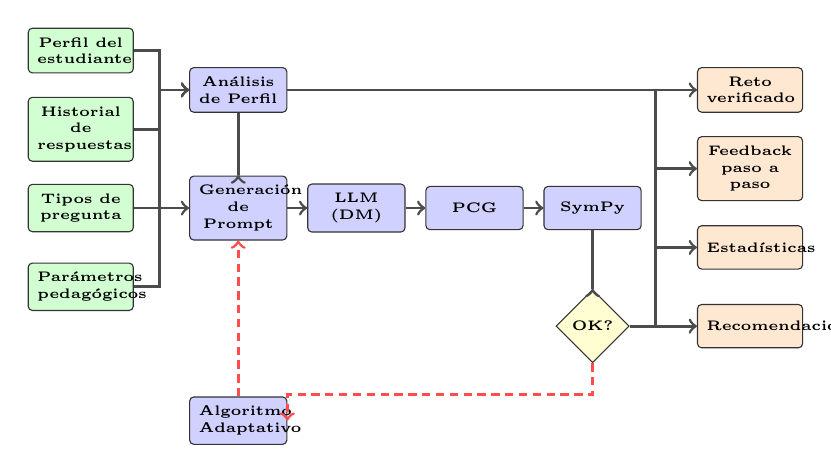
\begin{tikzpicture}[
  entry_node/.style={rectangle, draw=black!80, fill=green!18, text width=1.1cm, text centered, font=\tiny\bfseries, rounded corners=1.5pt, minimum height=0.55cm},
  process_node/.style={rectangle, draw=black!80, fill=blue!18, text width=1.0cm, text centered, font=\tiny\bfseries, rounded corners=1.5pt, minimum height=0.55cm},
  decision_node/.style={diamond, draw=black!80, fill=yellow!18, inner sep=2pt, font=\tiny\bfseries},
  output_node/.style={rectangle, draw=black!80, fill=orange!18, text width=1.1cm, text centered, font=\tiny\bfseries, rounded corners=1.5pt, minimum height=0.55cm},
  arrow/.style={->, line width=1pt, color=black!70},
  feedback_arrow/.style={->, line width=1pt, color=red!70, densely dashed},
]

% ENTRADAS (Columna 1)
\node [entry_node] at (0, 3.2) (in1) {Perfil del\\estudiante};
\node [entry_node] at (0, 2.2) (in2) {Historial de\\respuestas};
\node [entry_node] at (0, 1.2) (in3) {Tipos de\\pregunta};
\node [entry_node] at (0, 0.2) (in4) {Parámetros\\pedagógicos};

% ANÁLISIS (Columna 2A)
\node [process_node] at (2.0, 2.7) (analisis) {Análisis\\de Perfil};

% GENERACIÓN DE PROMPT (Columna 2B)
\node [process_node] at (2.0, 1.2) (prompt) {Generación\\de Prompt};

% PROCESAMIENTO CENTRAL (Columna 3-4)
\node [process_node] at (3.5, 1.2) (llm) {LLM (DM)};
\node [process_node] at (5.0, 1.2) (pcg) {PCG};
\node [process_node] at (6.5, 1.2) (sympy) {SymPy};
\node [decision_node] at (6.5, -0.3) (check) {OK?};

% ADAPTACIÓN (Columna 2 - abajo)
\node [process_node] at (2.0, -1.5) (adapt) {Algoritmo\\Adaptativo};

% SALIDAS (Columna 5)
\node [output_node] at (8.5, 2.7) (out1) {Reto\\verificado};
\node [output_node] at (8.5, 1.7) (out2) {Feedback\\paso a paso};
\node [output_node] at (8.5, 0.7) (out3) {Estadísticas};
\node [output_node] at (8.5, -0.3) (out4) {Recomendaciones};

% ============ CONEXIONES ENTRADAS → PROCESOS ============
% Perfil, Historial, Parámetros → Análisis
\draw [arrow] (in1.east) -- (1.0, 3.2) -- (1.0, 2.7) -- (analisis.west);
\draw [arrow] (in2.east) -- (1.0, 2.2) -- (1.0, 2.7) -- (analisis.west);
\draw [arrow] (in4.east) -- (1.0, 0.2) -- (1.0, 2.7) -- (analisis.west);

% Tipos de pregunta → Prompt
\draw [arrow] (in3.east) -- (1.0, 1.2) -- (prompt.west);

% Análisis → Prompt
\draw [arrow] (analisis.south) -- (analisis.south |- prompt.north) -- (prompt.north);

% ============ CONEXIONES PROCESOS CENTRALES ============
% Prompt → LLM
\draw [arrow] (prompt.east) -- (llm.west);
% LLM → PCG
\draw [arrow] (llm.east) -- (pcg.west);
% PCG → SymPy
\draw [arrow] (pcg.east) -- (sympy.west);
% SymPy → Decision
\draw [arrow] (sympy.south) -- (sympy.south |- check.north) -- (check.north);

% ============ BUCLE DE RETROALIMENTACIÓN (NO) ============
% Check → Adapt
\draw [feedback_arrow] (check.south) -- ++(0,-0.4) -| (adapt.east);
% Adapt → Prompt (retroalimentación ortogonal)
\draw [feedback_arrow] (adapt.north) -- ++(0,0.4) -| (prompt.south);

% ============ CONEXIONES A SALIDAS (SÍ) ============
% Check → Reto verificado
\draw [arrow] (check.east) -- (7.3, -0.3) -- (7.3, 2.7) -- (out1.west);

% Check → Feedback paso a paso
\draw [arrow] (check.east) -- (7.3, -0.3) -- (7.3, 1.7) -- (out2.west);

% Análisis → Estadísticas (información de contexto)
\draw [arrow] (analisis.east) -- (7.3, 2.7) -- (7.3, 0.7) -- (out3.west);

% Check → Recomendaciones
\draw [arrow] (check.east) -- (7.3, -0.3) -- (out4.west);

\end{tikzpicture}%
}
\caption{Diagrama de caja gris de LUCID: arquitectura de sistemas con flujo de información ortogonal. Entradas individuales (verde) fluyen hacia procesos específicos (azul), pasando por validación SymPy con decisión (amarillo). El bucle de retroalimentación rojo (punteado) maneja fallos de validación. Salidas diferenciadas (naranja) se generan según el estado del sistema.}
\label{fig:architecture}
\end{figure}
  
El sistema opera bajo el siguiente flujo secuencial de procesamiento:

\paragraph{Paso 1 - Análisis de Perfil:} Se recuperan e integran el perfil del estudiante (dominio actual, tasa de éxito), el historial de respuestas anteriores y los parámetros pedagógicos configurados. Este análisis multidimensional construye el modelo conceptual actual del aprendiz, incluyendo brechas de conocimiento y patrones de error.

\paragraph{Paso 2 - Generación de Directiva Contextualizada:} El análisis de perfil se combina con los tipos de pregunta seleccionados para generar un prompt dinámico que instruye al LLM a asumir el rol de ``Dungeon Master'' pedagógico. Este prompt inyecta metadatos de contexto (nivel conceptual, restricciones narrativas, tipos de operaciones esperadas) en una plantilla reutilizable que asegura coherencia entre iteraciones.

\paragraph{Paso 3 - Síntesis LLM (Dungeon Master):} El modelo de lenguaje generativo sintetiza un reto narrativo cohesivo que integra tanto el texto narrativo como la expresión matemática del problema. El LLM actúa como motor creativo, garantizando que el desafío sea pedagógicamente relevante y narrativamente inmersivo.

\paragraph{Paso 4 - Generación Procedural de Contenido (PCG):} La salida del LLM se parsea estructuradamente para extraer el núcleo matemático (operaciones, restricciones, soluciones posibles) y se inserta en la mecánica interactiva del entorno de juego, transformando la narrativa en un reto jugable.

\paragraph{Paso 5 - Validación Simbólica (SymPy):} Un microservicio Python/SymPy ejecuta validación determinista, verificando que la matemática sea correcta, que no haya alucinaciones en la expresión, y que el reto sea resoluble bajo las restricciones pedagógicas especificadas.

\paragraph{Paso 6 - Decisión Adaptativa y Cierre:} Si la validación es exitosa (OK = Sí), el reto verificado se entrega al estudiante junto con el feedback paso a paso, estadísticas de contexto y recomendaciones personalizadas. Si falla (OK = No), el Algoritmo Adaptativo reajusta parámetros pedagógicos (reduce complejidad, añade analogías, modifica restricciones) y reinicia desde Paso 2, garantizando convergencia hacia retos válidos.

Esta arquitectura de dos capas con validación determinística separa claramente la responsabilidad de coherencia narrativa (LLM) del ``oráculo de verdad'' matemática (SymPy), garantizando que cada estudiante solo enfrenta desafíos que son simultáneamente pedagógicamente íntegros, narrativamente significativos y matemáticamente correctos.

\bibliographystyle{IEEEtran}
\bibliography{ref}

\vfill\pagebreak

\end{document}
